\documentclass[11pt]{article}

    \usepackage[breakable]{tcolorbox}
    \usepackage{parskip} % Stop auto-indenting (to mimic markdown behaviour)
    
    \usepackage{iftex}
    \ifPDFTeX
    	\usepackage[T1]{fontenc}
    	\usepackage{mathpazo}
    \else
    	\usepackage{fontspec}
    \fi

    % Basic figure setup, for now with no caption control since it's done
    % automatically by Pandoc (which extracts ![](path) syntax from Markdown).
    \usepackage{graphicx}
    % Maintain compatibility with old templates. Remove in nbconvert 6.0
    \let\Oldincludegraphics\includegraphics
    % Ensure that by default, figures have no caption (until we provide a
    % proper Figure object with a Caption API and a way to capture that
    % in the conversion process - todo).
    \usepackage{caption}
    \DeclareCaptionFormat{nocaption}{}
    \captionsetup{format=nocaption,aboveskip=0pt,belowskip=0pt}

    \usepackage{float}
    \floatplacement{figure}{H} % forces figures to be placed at the correct location
    \usepackage{xcolor} % Allow colors to be defined
    \usepackage{enumerate} % Needed for markdown enumerations to work
    \usepackage{geometry} % Used to adjust the document margins
    \usepackage{amsmath} % Equations
    \usepackage{amssymb} % Equations
    \usepackage{textcomp} % defines textquotesingle
    % Hack from http://tex.stackexchange.com/a/47451/13684:
    \AtBeginDocument{%
        \def\PYZsq{\textquotesingle}% Upright quotes in Pygmentized code
    }
    \usepackage{upquote} % Upright quotes for verbatim code
    \usepackage{eurosym} % defines \euro
    \usepackage[mathletters]{ucs} % Extended unicode (utf-8) support
    \usepackage{fancyvrb} % verbatim replacement that allows latex
    \usepackage{grffile} % extends the file name processing of package graphics 
                         % to support a larger range
    \makeatletter % fix for old versions of grffile with XeLaTeX
    \@ifpackagelater{grffile}{2019/11/01}
    {
      % Do nothing on new versions
    }
    {
      \def\Gread@@xetex#1{%
        \IfFileExists{"\Gin@base".bb}%
        {\Gread@eps{\Gin@base.bb}}%
        {\Gread@@xetex@aux#1}%
      }
    }
    \makeatother
    \usepackage[Export]{adjustbox} % Used to constrain images to a maximum size
    \adjustboxset{max size={0.9\linewidth}{0.9\paperheight}}

    % The hyperref package gives us a pdf with properly built
    % internal navigation ('pdf bookmarks' for the table of contents,
    % internal cross-reference links, web links for URLs, etc.)
    \usepackage{hyperref}
    % The default LaTeX title has an obnoxious amount of whitespace. By default,
    % titling removes some of it. It also provides customization options.
    \usepackage{titling}
    \usepackage{longtable} % longtable support required by pandoc >1.10
    \usepackage{booktabs}  % table support for pandoc > 1.12.2
    \usepackage[inline]{enumitem} % IRkernel/repr support (it uses the enumerate* environment)
    \usepackage[normalem]{ulem} % ulem is needed to support strikethroughs (\sout)
                                % normalem makes italics be italics, not underlines
    \usepackage{mathrsfs}
    

    
    % Colors for the hyperref package
    \definecolor{urlcolor}{rgb}{0,.145,.698}
    \definecolor{linkcolor}{rgb}{.71,0.21,0.01}
    \definecolor{citecolor}{rgb}{.12,.54,.11}

    % ANSI colors
    \definecolor{ansi-black}{HTML}{3E424D}
    \definecolor{ansi-black-intense}{HTML}{282C36}
    \definecolor{ansi-red}{HTML}{E75C58}
    \definecolor{ansi-red-intense}{HTML}{B22B31}
    \definecolor{ansi-green}{HTML}{00A250}
    \definecolor{ansi-green-intense}{HTML}{007427}
    \definecolor{ansi-yellow}{HTML}{DDB62B}
    \definecolor{ansi-yellow-intense}{HTML}{B27D12}
    \definecolor{ansi-blue}{HTML}{208FFB}
    \definecolor{ansi-blue-intense}{HTML}{0065CA}
    \definecolor{ansi-magenta}{HTML}{D160C4}
    \definecolor{ansi-magenta-intense}{HTML}{A03196}
    \definecolor{ansi-cyan}{HTML}{60C6C8}
    \definecolor{ansi-cyan-intense}{HTML}{258F8F}
    \definecolor{ansi-white}{HTML}{C5C1B4}
    \definecolor{ansi-white-intense}{HTML}{A1A6B2}
    \definecolor{ansi-default-inverse-fg}{HTML}{FFFFFF}
    \definecolor{ansi-default-inverse-bg}{HTML}{000000}

    % common color for the border for error outputs.
    \definecolor{outerrorbackground}{HTML}{FFDFDF}

    % commands and environments needed by pandoc snippets
    % extracted from the output of `pandoc -s`
    \providecommand{\tightlist}{%
      \setlength{\itemsep}{0pt}\setlength{\parskip}{0pt}}
    \DefineVerbatimEnvironment{Highlighting}{Verbatim}{commandchars=\\\{\}}
    % Add ',fontsize=\small' for more characters per line
    \newenvironment{Shaded}{}{}
    \newcommand{\KeywordTok}[1]{\textcolor[rgb]{0.00,0.44,0.13}{\textbf{{#1}}}}
    \newcommand{\DataTypeTok}[1]{\textcolor[rgb]{0.56,0.13,0.00}{{#1}}}
    \newcommand{\DecValTok}[1]{\textcolor[rgb]{0.25,0.63,0.44}{{#1}}}
    \newcommand{\BaseNTok}[1]{\textcolor[rgb]{0.25,0.63,0.44}{{#1}}}
    \newcommand{\FloatTok}[1]{\textcolor[rgb]{0.25,0.63,0.44}{{#1}}}
    \newcommand{\CharTok}[1]{\textcolor[rgb]{0.25,0.44,0.63}{{#1}}}
    \newcommand{\StringTok}[1]{\textcolor[rgb]{0.25,0.44,0.63}{{#1}}}
    \newcommand{\CommentTok}[1]{\textcolor[rgb]{0.38,0.63,0.69}{\textit{{#1}}}}
    \newcommand{\OtherTok}[1]{\textcolor[rgb]{0.00,0.44,0.13}{{#1}}}
    \newcommand{\AlertTok}[1]{\textcolor[rgb]{1.00,0.00,0.00}{\textbf{{#1}}}}
    \newcommand{\FunctionTok}[1]{\textcolor[rgb]{0.02,0.16,0.49}{{#1}}}
    \newcommand{\RegionMarkerTok}[1]{{#1}}
    \newcommand{\ErrorTok}[1]{\textcolor[rgb]{1.00,0.00,0.00}{\textbf{{#1}}}}
    \newcommand{\NormalTok}[1]{{#1}}
    
    % Additional commands for more recent versions of Pandoc
    \newcommand{\ConstantTok}[1]{\textcolor[rgb]{0.53,0.00,0.00}{{#1}}}
    \newcommand{\SpecialCharTok}[1]{\textcolor[rgb]{0.25,0.44,0.63}{{#1}}}
    \newcommand{\VerbatimStringTok}[1]{\textcolor[rgb]{0.25,0.44,0.63}{{#1}}}
    \newcommand{\SpecialStringTok}[1]{\textcolor[rgb]{0.73,0.40,0.53}{{#1}}}
    \newcommand{\ImportTok}[1]{{#1}}
    \newcommand{\DocumentationTok}[1]{\textcolor[rgb]{0.73,0.13,0.13}{\textit{{#1}}}}
    \newcommand{\AnnotationTok}[1]{\textcolor[rgb]{0.38,0.63,0.69}{\textbf{\textit{{#1}}}}}
    \newcommand{\CommentVarTok}[1]{\textcolor[rgb]{0.38,0.63,0.69}{\textbf{\textit{{#1}}}}}
    \newcommand{\VariableTok}[1]{\textcolor[rgb]{0.10,0.09,0.49}{{#1}}}
    \newcommand{\ControlFlowTok}[1]{\textcolor[rgb]{0.00,0.44,0.13}{\textbf{{#1}}}}
    \newcommand{\OperatorTok}[1]{\textcolor[rgb]{0.40,0.40,0.40}{{#1}}}
    \newcommand{\BuiltInTok}[1]{{#1}}
    \newcommand{\ExtensionTok}[1]{{#1}}
    \newcommand{\PreprocessorTok}[1]{\textcolor[rgb]{0.74,0.48,0.00}{{#1}}}
    \newcommand{\AttributeTok}[1]{\textcolor[rgb]{0.49,0.56,0.16}{{#1}}}
    \newcommand{\InformationTok}[1]{\textcolor[rgb]{0.38,0.63,0.69}{\textbf{\textit{{#1}}}}}
    \newcommand{\WarningTok}[1]{\textcolor[rgb]{0.38,0.63,0.69}{\textbf{\textit{{#1}}}}}
    
    
    % Define a nice break command that doesn't care if a line doesn't already
    % exist.
    \def\br{\hspace*{\fill} \\* }
    % Math Jax compatibility definitions
    \def\gt{>}
    \def\lt{<}
    \let\Oldtex\TeX
    \let\Oldlatex\LaTeX
    \renewcommand{\TeX}{\textrm{\Oldtex}}
    \renewcommand{\LaTeX}{\textrm{\Oldlatex}}
    % Document parameters
    % Document title
    \title{chapter-4-4}
    
    
    
    
    
% Pygments definitions
\makeatletter
\def\PY@reset{\let\PY@it=\relax \let\PY@bf=\relax%
    \let\PY@ul=\relax \let\PY@tc=\relax%
    \let\PY@bc=\relax \let\PY@ff=\relax}
\def\PY@tok#1{\csname PY@tok@#1\endcsname}
\def\PY@toks#1+{\ifx\relax#1\empty\else%
    \PY@tok{#1}\expandafter\PY@toks\fi}
\def\PY@do#1{\PY@bc{\PY@tc{\PY@ul{%
    \PY@it{\PY@bf{\PY@ff{#1}}}}}}}
\def\PY#1#2{\PY@reset\PY@toks#1+\relax+\PY@do{#2}}

\@namedef{PY@tok@w}{\def\PY@tc##1{\textcolor[rgb]{0.73,0.73,0.73}{##1}}}
\@namedef{PY@tok@c}{\let\PY@it=\textit\def\PY@tc##1{\textcolor[rgb]{0.25,0.50,0.50}{##1}}}
\@namedef{PY@tok@cp}{\def\PY@tc##1{\textcolor[rgb]{0.74,0.48,0.00}{##1}}}
\@namedef{PY@tok@k}{\let\PY@bf=\textbf\def\PY@tc##1{\textcolor[rgb]{0.00,0.50,0.00}{##1}}}
\@namedef{PY@tok@kp}{\def\PY@tc##1{\textcolor[rgb]{0.00,0.50,0.00}{##1}}}
\@namedef{PY@tok@kt}{\def\PY@tc##1{\textcolor[rgb]{0.69,0.00,0.25}{##1}}}
\@namedef{PY@tok@o}{\def\PY@tc##1{\textcolor[rgb]{0.40,0.40,0.40}{##1}}}
\@namedef{PY@tok@ow}{\let\PY@bf=\textbf\def\PY@tc##1{\textcolor[rgb]{0.67,0.13,1.00}{##1}}}
\@namedef{PY@tok@nb}{\def\PY@tc##1{\textcolor[rgb]{0.00,0.50,0.00}{##1}}}
\@namedef{PY@tok@nf}{\def\PY@tc##1{\textcolor[rgb]{0.00,0.00,1.00}{##1}}}
\@namedef{PY@tok@nc}{\let\PY@bf=\textbf\def\PY@tc##1{\textcolor[rgb]{0.00,0.00,1.00}{##1}}}
\@namedef{PY@tok@nn}{\let\PY@bf=\textbf\def\PY@tc##1{\textcolor[rgb]{0.00,0.00,1.00}{##1}}}
\@namedef{PY@tok@ne}{\let\PY@bf=\textbf\def\PY@tc##1{\textcolor[rgb]{0.82,0.25,0.23}{##1}}}
\@namedef{PY@tok@nv}{\def\PY@tc##1{\textcolor[rgb]{0.10,0.09,0.49}{##1}}}
\@namedef{PY@tok@no}{\def\PY@tc##1{\textcolor[rgb]{0.53,0.00,0.00}{##1}}}
\@namedef{PY@tok@nl}{\def\PY@tc##1{\textcolor[rgb]{0.63,0.63,0.00}{##1}}}
\@namedef{PY@tok@ni}{\let\PY@bf=\textbf\def\PY@tc##1{\textcolor[rgb]{0.60,0.60,0.60}{##1}}}
\@namedef{PY@tok@na}{\def\PY@tc##1{\textcolor[rgb]{0.49,0.56,0.16}{##1}}}
\@namedef{PY@tok@nt}{\let\PY@bf=\textbf\def\PY@tc##1{\textcolor[rgb]{0.00,0.50,0.00}{##1}}}
\@namedef{PY@tok@nd}{\def\PY@tc##1{\textcolor[rgb]{0.67,0.13,1.00}{##1}}}
\@namedef{PY@tok@s}{\def\PY@tc##1{\textcolor[rgb]{0.73,0.13,0.13}{##1}}}
\@namedef{PY@tok@sd}{\let\PY@it=\textit\def\PY@tc##1{\textcolor[rgb]{0.73,0.13,0.13}{##1}}}
\@namedef{PY@tok@si}{\let\PY@bf=\textbf\def\PY@tc##1{\textcolor[rgb]{0.73,0.40,0.53}{##1}}}
\@namedef{PY@tok@se}{\let\PY@bf=\textbf\def\PY@tc##1{\textcolor[rgb]{0.73,0.40,0.13}{##1}}}
\@namedef{PY@tok@sr}{\def\PY@tc##1{\textcolor[rgb]{0.73,0.40,0.53}{##1}}}
\@namedef{PY@tok@ss}{\def\PY@tc##1{\textcolor[rgb]{0.10,0.09,0.49}{##1}}}
\@namedef{PY@tok@sx}{\def\PY@tc##1{\textcolor[rgb]{0.00,0.50,0.00}{##1}}}
\@namedef{PY@tok@m}{\def\PY@tc##1{\textcolor[rgb]{0.40,0.40,0.40}{##1}}}
\@namedef{PY@tok@gh}{\let\PY@bf=\textbf\def\PY@tc##1{\textcolor[rgb]{0.00,0.00,0.50}{##1}}}
\@namedef{PY@tok@gu}{\let\PY@bf=\textbf\def\PY@tc##1{\textcolor[rgb]{0.50,0.00,0.50}{##1}}}
\@namedef{PY@tok@gd}{\def\PY@tc##1{\textcolor[rgb]{0.63,0.00,0.00}{##1}}}
\@namedef{PY@tok@gi}{\def\PY@tc##1{\textcolor[rgb]{0.00,0.63,0.00}{##1}}}
\@namedef{PY@tok@gr}{\def\PY@tc##1{\textcolor[rgb]{1.00,0.00,0.00}{##1}}}
\@namedef{PY@tok@ge}{\let\PY@it=\textit}
\@namedef{PY@tok@gs}{\let\PY@bf=\textbf}
\@namedef{PY@tok@gp}{\let\PY@bf=\textbf\def\PY@tc##1{\textcolor[rgb]{0.00,0.00,0.50}{##1}}}
\@namedef{PY@tok@go}{\def\PY@tc##1{\textcolor[rgb]{0.53,0.53,0.53}{##1}}}
\@namedef{PY@tok@gt}{\def\PY@tc##1{\textcolor[rgb]{0.00,0.27,0.87}{##1}}}
\@namedef{PY@tok@err}{\def\PY@bc##1{{\setlength{\fboxsep}{\string -\fboxrule}\fcolorbox[rgb]{1.00,0.00,0.00}{1,1,1}{\strut ##1}}}}
\@namedef{PY@tok@kc}{\let\PY@bf=\textbf\def\PY@tc##1{\textcolor[rgb]{0.00,0.50,0.00}{##1}}}
\@namedef{PY@tok@kd}{\let\PY@bf=\textbf\def\PY@tc##1{\textcolor[rgb]{0.00,0.50,0.00}{##1}}}
\@namedef{PY@tok@kn}{\let\PY@bf=\textbf\def\PY@tc##1{\textcolor[rgb]{0.00,0.50,0.00}{##1}}}
\@namedef{PY@tok@kr}{\let\PY@bf=\textbf\def\PY@tc##1{\textcolor[rgb]{0.00,0.50,0.00}{##1}}}
\@namedef{PY@tok@bp}{\def\PY@tc##1{\textcolor[rgb]{0.00,0.50,0.00}{##1}}}
\@namedef{PY@tok@fm}{\def\PY@tc##1{\textcolor[rgb]{0.00,0.00,1.00}{##1}}}
\@namedef{PY@tok@vc}{\def\PY@tc##1{\textcolor[rgb]{0.10,0.09,0.49}{##1}}}
\@namedef{PY@tok@vg}{\def\PY@tc##1{\textcolor[rgb]{0.10,0.09,0.49}{##1}}}
\@namedef{PY@tok@vi}{\def\PY@tc##1{\textcolor[rgb]{0.10,0.09,0.49}{##1}}}
\@namedef{PY@tok@vm}{\def\PY@tc##1{\textcolor[rgb]{0.10,0.09,0.49}{##1}}}
\@namedef{PY@tok@sa}{\def\PY@tc##1{\textcolor[rgb]{0.73,0.13,0.13}{##1}}}
\@namedef{PY@tok@sb}{\def\PY@tc##1{\textcolor[rgb]{0.73,0.13,0.13}{##1}}}
\@namedef{PY@tok@sc}{\def\PY@tc##1{\textcolor[rgb]{0.73,0.13,0.13}{##1}}}
\@namedef{PY@tok@dl}{\def\PY@tc##1{\textcolor[rgb]{0.73,0.13,0.13}{##1}}}
\@namedef{PY@tok@s2}{\def\PY@tc##1{\textcolor[rgb]{0.73,0.13,0.13}{##1}}}
\@namedef{PY@tok@sh}{\def\PY@tc##1{\textcolor[rgb]{0.73,0.13,0.13}{##1}}}
\@namedef{PY@tok@s1}{\def\PY@tc##1{\textcolor[rgb]{0.73,0.13,0.13}{##1}}}
\@namedef{PY@tok@mb}{\def\PY@tc##1{\textcolor[rgb]{0.40,0.40,0.40}{##1}}}
\@namedef{PY@tok@mf}{\def\PY@tc##1{\textcolor[rgb]{0.40,0.40,0.40}{##1}}}
\@namedef{PY@tok@mh}{\def\PY@tc##1{\textcolor[rgb]{0.40,0.40,0.40}{##1}}}
\@namedef{PY@tok@mi}{\def\PY@tc##1{\textcolor[rgb]{0.40,0.40,0.40}{##1}}}
\@namedef{PY@tok@il}{\def\PY@tc##1{\textcolor[rgb]{0.40,0.40,0.40}{##1}}}
\@namedef{PY@tok@mo}{\def\PY@tc##1{\textcolor[rgb]{0.40,0.40,0.40}{##1}}}
\@namedef{PY@tok@ch}{\let\PY@it=\textit\def\PY@tc##1{\textcolor[rgb]{0.25,0.50,0.50}{##1}}}
\@namedef{PY@tok@cm}{\let\PY@it=\textit\def\PY@tc##1{\textcolor[rgb]{0.25,0.50,0.50}{##1}}}
\@namedef{PY@tok@cpf}{\let\PY@it=\textit\def\PY@tc##1{\textcolor[rgb]{0.25,0.50,0.50}{##1}}}
\@namedef{PY@tok@c1}{\let\PY@it=\textit\def\PY@tc##1{\textcolor[rgb]{0.25,0.50,0.50}{##1}}}
\@namedef{PY@tok@cs}{\let\PY@it=\textit\def\PY@tc##1{\textcolor[rgb]{0.25,0.50,0.50}{##1}}}

\def\PYZbs{\char`\\}
\def\PYZus{\char`\_}
\def\PYZob{\char`\{}
\def\PYZcb{\char`\}}
\def\PYZca{\char`\^}
\def\PYZam{\char`\&}
\def\PYZlt{\char`\<}
\def\PYZgt{\char`\>}
\def\PYZsh{\char`\#}
\def\PYZpc{\char`\%}
\def\PYZdl{\char`\$}
\def\PYZhy{\char`\-}
\def\PYZsq{\char`\'}
\def\PYZdq{\char`\"}
\def\PYZti{\char`\~}
% for compatibility with earlier versions
\def\PYZat{@}
\def\PYZlb{[}
\def\PYZrb{]}
\makeatother


    % For linebreaks inside Verbatim environment from package fancyvrb. 
    \makeatletter
        \newbox\Wrappedcontinuationbox 
        \newbox\Wrappedvisiblespacebox 
        \newcommand*\Wrappedvisiblespace {\textcolor{red}{\textvisiblespace}} 
        \newcommand*\Wrappedcontinuationsymbol {\textcolor{red}{\llap{\tiny$\m@th\hookrightarrow$}}} 
        \newcommand*\Wrappedcontinuationindent {3ex } 
        \newcommand*\Wrappedafterbreak {\kern\Wrappedcontinuationindent\copy\Wrappedcontinuationbox} 
        % Take advantage of the already applied Pygments mark-up to insert 
        % potential linebreaks for TeX processing. 
        %        {, <, #, %, $, ' and ": go to next line. 
        %        _, }, ^, &, >, - and ~: stay at end of broken line. 
        % Use of \textquotesingle for straight quote. 
        \newcommand*\Wrappedbreaksatspecials {% 
            \def\PYGZus{\discretionary{\char`\_}{\Wrappedafterbreak}{\char`\_}}% 
            \def\PYGZob{\discretionary{}{\Wrappedafterbreak\char`\{}{\char`\{}}% 
            \def\PYGZcb{\discretionary{\char`\}}{\Wrappedafterbreak}{\char`\}}}% 
            \def\PYGZca{\discretionary{\char`\^}{\Wrappedafterbreak}{\char`\^}}% 
            \def\PYGZam{\discretionary{\char`\&}{\Wrappedafterbreak}{\char`\&}}% 
            \def\PYGZlt{\discretionary{}{\Wrappedafterbreak\char`\<}{\char`\<}}% 
            \def\PYGZgt{\discretionary{\char`\>}{\Wrappedafterbreak}{\char`\>}}% 
            \def\PYGZsh{\discretionary{}{\Wrappedafterbreak\char`\#}{\char`\#}}% 
            \def\PYGZpc{\discretionary{}{\Wrappedafterbreak\char`\%}{\char`\%}}% 
            \def\PYGZdl{\discretionary{}{\Wrappedafterbreak\char`\$}{\char`\$}}% 
            \def\PYGZhy{\discretionary{\char`\-}{\Wrappedafterbreak}{\char`\-}}% 
            \def\PYGZsq{\discretionary{}{\Wrappedafterbreak\textquotesingle}{\textquotesingle}}% 
            \def\PYGZdq{\discretionary{}{\Wrappedafterbreak\char`\"}{\char`\"}}% 
            \def\PYGZti{\discretionary{\char`\~}{\Wrappedafterbreak}{\char`\~}}% 
        } 
        % Some characters . , ; ? ! / are not pygmentized. 
        % This macro makes them "active" and they will insert potential linebreaks 
        \newcommand*\Wrappedbreaksatpunct {% 
            \lccode`\~`\.\lowercase{\def~}{\discretionary{\hbox{\char`\.}}{\Wrappedafterbreak}{\hbox{\char`\.}}}% 
            \lccode`\~`\,\lowercase{\def~}{\discretionary{\hbox{\char`\,}}{\Wrappedafterbreak}{\hbox{\char`\,}}}% 
            \lccode`\~`\;\lowercase{\def~}{\discretionary{\hbox{\char`\;}}{\Wrappedafterbreak}{\hbox{\char`\;}}}% 
            \lccode`\~`\:\lowercase{\def~}{\discretionary{\hbox{\char`\:}}{\Wrappedafterbreak}{\hbox{\char`\:}}}% 
            \lccode`\~`\?\lowercase{\def~}{\discretionary{\hbox{\char`\?}}{\Wrappedafterbreak}{\hbox{\char`\?}}}% 
            \lccode`\~`\!\lowercase{\def~}{\discretionary{\hbox{\char`\!}}{\Wrappedafterbreak}{\hbox{\char`\!}}}% 
            \lccode`\~`\/\lowercase{\def~}{\discretionary{\hbox{\char`\/}}{\Wrappedafterbreak}{\hbox{\char`\/}}}% 
            \catcode`\.\active
            \catcode`\,\active 
            \catcode`\;\active
            \catcode`\:\active
            \catcode`\?\active
            \catcode`\!\active
            \catcode`\/\active 
            \lccode`\~`\~ 	
        }
    \makeatother

    \let\OriginalVerbatim=\Verbatim
    \makeatletter
    \renewcommand{\Verbatim}[1][1]{%
        %\parskip\z@skip
        \sbox\Wrappedcontinuationbox {\Wrappedcontinuationsymbol}%
        \sbox\Wrappedvisiblespacebox {\FV@SetupFont\Wrappedvisiblespace}%
        \def\FancyVerbFormatLine ##1{\hsize\linewidth
            \vtop{\raggedright\hyphenpenalty\z@\exhyphenpenalty\z@
                \doublehyphendemerits\z@\finalhyphendemerits\z@
                \strut ##1\strut}%
        }%
        % If the linebreak is at a space, the latter will be displayed as visible
        % space at end of first line, and a continuation symbol starts next line.
        % Stretch/shrink are however usually zero for typewriter font.
        \def\FV@Space {%
            \nobreak\hskip\z@ plus\fontdimen3\font minus\fontdimen4\font
            \discretionary{\copy\Wrappedvisiblespacebox}{\Wrappedafterbreak}
            {\kern\fontdimen2\font}%
        }%
        
        % Allow breaks at special characters using \PYG... macros.
        \Wrappedbreaksatspecials
        % Breaks at punctuation characters . , ; ? ! and / need catcode=\active 	
        \OriginalVerbatim[#1,codes*=\Wrappedbreaksatpunct]%
    }
    \makeatother

    % Exact colors from NB
    \definecolor{incolor}{HTML}{303F9F}
    \definecolor{outcolor}{HTML}{D84315}
    \definecolor{cellborder}{HTML}{CFCFCF}
    \definecolor{cellbackground}{HTML}{F7F7F7}
    
    % prompt
    \makeatletter
    \newcommand{\boxspacing}{\kern\kvtcb@left@rule\kern\kvtcb@boxsep}
    \makeatother
    \newcommand{\prompt}[4]{
        {\ttfamily\llap{{\color{#2}[#3]:\hspace{3pt}#4}}\vspace{-\baselineskip}}
    }
    

    
    % Prevent overflowing lines due to hard-to-break entities
    \sloppy 
    % Setup hyperref package
    \hypersetup{
      breaklinks=true,  % so long urls are correctly broken across lines
      colorlinks=true,
      urlcolor=urlcolor,
      linkcolor=linkcolor,
      citecolor=citecolor,
      }
    % Slightly bigger margins than the latex defaults
    
    \geometry{verbose,tmargin=1in,bmargin=1in,lmargin=1in,rmargin=1in}
    
    

\begin{document}
    
    \maketitle
    
    

    
    \hypertarget{model-evaluation-and-hyperparameter-tuning}{%
\section{Model Evaluation and Hyperparameter
Tuning}\label{model-evaluation-and-hyperparameter-tuning}}

    \begin{quote}
\textbf{TODO} - Completare la parte sulle pipelines introducendo esempio
di Lewinson - Introdurre anche esempi sulla regressione logistica con
credito
\end{quote}

    In the previous chapters, you learned about the essential machine
learning algorithms for classification and how to get our data into
shape before we feed it into those algorithms. Now, it's time to learn
about the best practices of building good machine learning models by
fine-tuning the algorithms and evaluating the performance of the models.
In this chapter, we will learn how to do the following: - Assess the
performance of machine learning models - Diagnose the common problems of
machine learning algorithms - Fine-tune machine learning models -
Evaluate predictive models using different performance metrics

    \hypertarget{combining-transformers-and-estimators-in-a-pipeline}{%
\subsection{Combining Transformers and Estimators in a
Pipeline}\label{combining-transformers-and-estimators-in-a-pipeline}}

    \hypertarget{lets-make-a-simple-project-from-scratch}{%
\subsubsection{Let's make a simple project from scratch
\ldots{}}\label{lets-make-a-simple-project-from-scratch}}

    In this chapter, we tackle a binary classification problem set in the
financial industry. We work with a dataset contributed to the UCI
Machine Learning Repository (a very popular data repository). The
dataset used in this chapter was collected in a Taiwanese bank in
October 2005. The study was motivated by the fact that---at that
time---more and more banks were giving cash (and credit card) credit to
willing customers. You can download the sample file
\href{https://archive.ics.uci.edu/ml/datasets/default+of+credit+card+clients}{here}

    \begin{tcolorbox}[breakable, size=fbox, boxrule=1pt, pad at break*=1mm,colback=cellbackground, colframe=cellborder]
\prompt{In}{incolor}{27}{\boxspacing}
\begin{Verbatim}[commandchars=\\\{\}]
\PY{k+kn}{import} \PY{n+nn}{pandas} \PY{k}{as} \PY{n+nn}{pd}

\PY{k}{if} \PY{l+s+s1}{\PYZsq{}}\PY{l+s+s1}{google.colab}\PY{l+s+s1}{\PYZsq{}} \PY{o+ow}{in} \PY{n+nb}{str}\PY{p}{(}\PY{n}{get\PYZus{}ipython}\PY{p}{(}\PY{p}{)}\PY{p}{)}\PY{p}{:}
    \PY{k+kn}{from} \PY{n+nn}{google}\PY{n+nn}{.}\PY{n+nn}{colab} \PY{k+kn}{import} \PY{n}{files}
    \PY{n}{uploaded} \PY{o}{=} \PY{n}{files}\PY{o}{.}\PY{n}{upload}\PY{p}{(}\PY{p}{)}
    \PY{n}{path} \PY{o}{=} \PY{l+s+s1}{\PYZsq{}}\PY{l+s+s1}{\PYZsq{}}
\PY{k}{else}\PY{p}{:}
    \PY{n}{path} \PY{o}{=} \PY{l+s+s1}{\PYZsq{}}\PY{l+s+s1}{./data/}\PY{l+s+s1}{\PYZsq{}}
\end{Verbatim}
\end{tcolorbox}

    \begin{tcolorbox}[breakable, size=fbox, boxrule=1pt, pad at break*=1mm,colback=cellbackground, colframe=cellborder]
\prompt{In}{incolor}{29}{\boxspacing}
\begin{Verbatim}[commandchars=\\\{\}]
\PY{n}{column\PYZus{}dtypes} \PY{o}{=} \PY{p}{\PYZob{}}\PY{l+s+s1}{\PYZsq{}}\PY{l+s+s1}{EDUCATION}\PY{l+s+s1}{\PYZsq{}}\PY{p}{:} \PY{l+s+s1}{\PYZsq{}}\PY{l+s+s1}{category}\PY{l+s+s1}{\PYZsq{}}\PY{p}{,}
\PY{l+s+s1}{\PYZsq{}}\PY{l+s+s1}{MARRIAGE}\PY{l+s+s1}{\PYZsq{}}\PY{p}{:} \PY{l+s+s1}{\PYZsq{}}\PY{l+s+s1}{category}\PY{l+s+s1}{\PYZsq{}}\PY{p}{,}
\PY{l+s+s1}{\PYZsq{}}\PY{l+s+s1}{SEX}\PY{l+s+s1}{\PYZsq{}}\PY{p}{:} \PY{l+s+s1}{\PYZsq{}}\PY{l+s+s1}{category}\PY{l+s+s1}{\PYZsq{}}\PY{p}{,}
\PY{l+s+s1}{\PYZsq{}}\PY{l+s+s1}{PAYMENT\PYZus{}STATUS\PYZus{}SEP}\PY{l+s+s1}{\PYZsq{}}\PY{p}{:} \PY{l+s+s1}{\PYZsq{}}\PY{l+s+s1}{category}\PY{l+s+s1}{\PYZsq{}}\PY{p}{,}
\PY{l+s+s1}{\PYZsq{}}\PY{l+s+s1}{PAYMENT\PYZus{}STATUS\PYZus{}AUG}\PY{l+s+s1}{\PYZsq{}}\PY{p}{:} \PY{l+s+s1}{\PYZsq{}}\PY{l+s+s1}{category}\PY{l+s+s1}{\PYZsq{}}\PY{p}{,}
\PY{l+s+s1}{\PYZsq{}}\PY{l+s+s1}{PAYMENT\PYZus{}STATUS\PYZus{}JUL}\PY{l+s+s1}{\PYZsq{}}\PY{p}{:} \PY{l+s+s1}{\PYZsq{}}\PY{l+s+s1}{category}\PY{l+s+s1}{\PYZsq{}}\PY{p}{,}
\PY{l+s+s1}{\PYZsq{}}\PY{l+s+s1}{PAYMENT\PYZus{}STATUS\PYZus{}JUN}\PY{l+s+s1}{\PYZsq{}}\PY{p}{:} \PY{l+s+s1}{\PYZsq{}}\PY{l+s+s1}{category}\PY{l+s+s1}{\PYZsq{}}\PY{p}{,}
\PY{l+s+s1}{\PYZsq{}}\PY{l+s+s1}{PAYMENT\PYZus{}STATUS\PYZus{}MAY}\PY{l+s+s1}{\PYZsq{}}\PY{p}{:} \PY{l+s+s1}{\PYZsq{}}\PY{l+s+s1}{category}\PY{l+s+s1}{\PYZsq{}}\PY{p}{,}
\PY{l+s+s1}{\PYZsq{}}\PY{l+s+s1}{PAYMENT\PYZus{}STATUS\PYZus{}APR}\PY{l+s+s1}{\PYZsq{}}\PY{p}{:} \PY{l+s+s1}{\PYZsq{}}\PY{l+s+s1}{category}\PY{l+s+s1}{\PYZsq{}}\PY{p}{\PYZcb{}}

\PY{n}{df} \PY{o}{=} \PY{n}{pd}\PY{o}{.}\PY{n}{read\PYZus{}csv}\PY{p}{(}\PY{n}{path} \PY{o}{+} \PY{l+s+s1}{\PYZsq{}}\PY{l+s+s1}{credit\PYZus{}card\PYZus{}default.csv}\PY{l+s+s1}{\PYZsq{}}\PY{p}{,} \PY{n}{index\PYZus{}col}\PY{o}{=}\PY{l+m+mi}{0}\PY{p}{,} \PY{n}{na\PYZus{}values}\PY{o}{=}\PY{l+s+s1}{\PYZsq{}}\PY{l+s+s1}{\PYZsq{}}\PY{p}{,} \PY{n}{dtype}\PY{o}{=}\PY{n}{column\PYZus{}dtypes}\PY{p}{,} \PY{n}{sep}\PY{o}{=}\PY{l+s+s1}{\PYZsq{}}\PY{l+s+s1}{,}\PY{l+s+s1}{\PYZsq{}}\PY{p}{)}
\PY{n}{df}\PY{o}{.}\PY{n}{head}\PY{p}{(}\PY{p}{)}
\end{Verbatim}
\end{tcolorbox}

            \begin{tcolorbox}[breakable, size=fbox, boxrule=.5pt, pad at break*=1mm, opacityfill=0]
\prompt{Out}{outcolor}{29}{\boxspacing}
\begin{Verbatim}[commandchars=\\\{\}]
   limit\_bal     sex   education marriage   age        payment\_status\_sep  \textbackslash{}
0      20000  Female  University  Married  24.0  Payment delayed 2 months
1     120000  Female  University   Single  26.0                Payed duly
2      90000  Female  University   Single  34.0                   Unknown
3      50000  Female  University  Married  37.0                   Unknown
4      50000    Male  University  Married  57.0                Payed duly

         payment\_status\_aug payment\_status\_jul payment\_status\_jun  \textbackslash{}
0  Payment delayed 2 months         Payed duly         Payed duly
1  Payment delayed 2 months            Unknown            Unknown
2                   Unknown            Unknown            Unknown
3                   Unknown            Unknown            Unknown
4                   Unknown         Payed duly            Unknown

  payment\_status\_may  {\ldots} bill\_statement\_jun  bill\_statement\_may  \textbackslash{}
0            Unknown  {\ldots}                  0                   0
1            Unknown  {\ldots}               3272                3455
2            Unknown  {\ldots}              14331               14948
3            Unknown  {\ldots}              28314               28959
4            Unknown  {\ldots}              20940               19146

   bill\_statement\_apr  previous\_payment\_sep  previous\_payment\_aug  \textbackslash{}
0                   0                     0                   689
1                3261                     0                  1000
2               15549                  1518                  1500
3               29547                  2000                  2019
4               19131                  2000                 36681

   previous\_payment\_jul  previous\_payment\_jun  previous\_payment\_may  \textbackslash{}
0                     0                     0                     0
1                  1000                  1000                     0
2                  1000                  1000                  1000
3                  1200                  1100                  1069
4                 10000                  9000                   689

   previous\_payment\_apr  default\_payment\_next\_month
0                     0                           1
1                  2000                           1
2                  5000                           0
3                  1000                           0
4                   679                           0

[5 rows x 24 columns]
\end{Verbatim}
\end{tcolorbox}
        
    \begin{tcolorbox}[breakable, size=fbox, boxrule=1pt, pad at break*=1mm,colback=cellbackground, colframe=cellborder]
\prompt{In}{incolor}{32}{\boxspacing}
\begin{Verbatim}[commandchars=\\\{\}]
\PY{n}{X} \PY{o}{=} \PY{n}{df}\PY{o}{.}\PY{n}{copy}\PY{p}{(}\PY{p}{)}
\PY{n}{y} \PY{o}{=} \PY{n}{X}\PY{o}{.}\PY{n}{pop}\PY{p}{(}\PY{l+s+s1}{\PYZsq{}}\PY{l+s+s1}{default\PYZus{}payment\PYZus{}next\PYZus{}month}\PY{l+s+s1}{\PYZsq{}}\PY{p}{)}
\end{Verbatim}
\end{tcolorbox}

    \begin{tcolorbox}[breakable, size=fbox, boxrule=1pt, pad at break*=1mm,colback=cellbackground, colframe=cellborder]
\prompt{In}{incolor}{33}{\boxspacing}
\begin{Verbatim}[commandchars=\\\{\}]
\PY{n}{df}\PY{o}{.}\PY{n}{describe}\PY{p}{(}\PY{p}{)}\PY{o}{.}\PY{n}{transpose}\PY{p}{(}\PY{p}{)}\PY{o}{.}\PY{n}{round}\PY{p}{(}\PY{l+m+mi}{2}\PY{p}{)}
\end{Verbatim}
\end{tcolorbox}

            \begin{tcolorbox}[breakable, size=fbox, boxrule=.5pt, pad at break*=1mm, opacityfill=0]
\prompt{Out}{outcolor}{33}{\boxspacing}
\begin{Verbatim}[commandchars=\\\{\}]
                              count       mean        std       min       25\%  \textbackslash{}
limit\_bal                   30000.0  167484.32  129747.66   10000.0  50000.00
age                         29850.0      35.49       9.22      21.0     28.00
bill\_statement\_sep          30000.0   51223.33   73635.86 -165580.0   3558.75
bill\_statement\_aug          30000.0   49179.08   71173.77  -69777.0   2984.75
bill\_statement\_jul          30000.0   47013.15   69349.39 -157264.0   2666.25
bill\_statement\_jun          30000.0   43262.95   64332.86 -170000.0   2326.75
bill\_statement\_may          30000.0   40311.40   60797.16  -81334.0   1763.00
bill\_statement\_apr          30000.0   38871.76   59554.11 -339603.0   1256.00
previous\_payment\_sep        30000.0    5663.58   16563.28       0.0   1000.00
previous\_payment\_aug        30000.0    5921.16   23040.87       0.0    833.00
previous\_payment\_jul        30000.0    5225.68   17606.96       0.0    390.00
previous\_payment\_jun        30000.0    4826.08   15666.16       0.0    296.00
previous\_payment\_may        30000.0    4799.39   15278.31       0.0    252.50
previous\_payment\_apr        30000.0    5215.50   17777.47       0.0    117.75
default\_payment\_next\_month  30000.0       0.22       0.42       0.0      0.00

                                 50\%        75\%        max
limit\_bal                   140000.0  240000.00  1000000.0
age                             34.0      41.00       79.0
bill\_statement\_sep           22381.5   67091.00   964511.0
bill\_statement\_aug           21200.0   64006.25   983931.0
bill\_statement\_jul           20088.5   60164.75  1664089.0
bill\_statement\_jun           19052.0   54506.00   891586.0
bill\_statement\_may           18104.5   50190.50   927171.0
bill\_statement\_apr           17071.0   49198.25   961664.0
previous\_payment\_sep          2100.0    5006.00   873552.0
previous\_payment\_aug          2009.0    5000.00  1684259.0
previous\_payment\_jul          1800.0    4505.00   896040.0
previous\_payment\_jun          1500.0    4013.25   621000.0
previous\_payment\_may          1500.0    4031.50   426529.0
previous\_payment\_apr          1500.0    4000.00   528666.0
default\_payment\_next\_month       0.0       0.00        1.0
\end{Verbatim}
\end{tcolorbox}
        
    \begin{tcolorbox}[breakable, size=fbox, boxrule=1pt, pad at break*=1mm,colback=cellbackground, colframe=cellborder]
\prompt{In}{incolor}{39}{\boxspacing}
\begin{Verbatim}[commandchars=\\\{\}]
\PY{k+kn}{import} \PY{n+nn}{warnings}
\PY{n}{warnings}\PY{o}{.}\PY{n}{simplefilter}\PY{p}{(}\PY{l+s+s1}{\PYZsq{}}\PY{l+s+s1}{ignore}\PY{l+s+s1}{\PYZsq{}}\PY{p}{)}

\PY{k+kn}{import} \PY{n+nn}{matplotlib}\PY{n+nn}{.}\PY{n+nn}{pyplot} \PY{k}{as} \PY{n+nn}{plt}
\PY{k+kn}{import} \PY{n+nn}{seaborn} \PY{k}{as} \PY{n+nn}{sns}
\PY{k+kn}{import} \PY{n+nn}{numpy} \PY{k}{as} \PY{n+nn}{np}

\PY{n}{fig}\PY{p}{,} \PY{n}{ax} \PY{o}{=} \PY{n}{plt}\PY{o}{.}\PY{n}{subplots}\PY{p}{(}\PY{p}{)}
\PY{n}{sns}\PY{o}{.}\PY{n}{distplot}\PY{p}{(}\PY{n}{df}\PY{o}{.}\PY{n}{loc}\PY{p}{[}\PY{n}{df}\PY{o}{.}\PY{n}{sex}\PY{o}{==}\PY{l+s+s1}{\PYZsq{}}\PY{l+s+s1}{Male}\PY{l+s+s1}{\PYZsq{}}\PY{p}{,} \PY{l+s+s1}{\PYZsq{}}\PY{l+s+s1}{age}\PY{l+s+s1}{\PYZsq{}}\PY{p}{]}\PY{o}{.}\PY{n}{dropna}\PY{p}{(}\PY{p}{)}\PY{p}{,}
    \PY{n}{hist}\PY{o}{=}\PY{k+kc}{False}\PY{p}{,} \PY{n}{color}\PY{o}{=}\PY{l+s+s1}{\PYZsq{}}\PY{l+s+s1}{green}\PY{l+s+s1}{\PYZsq{}}\PY{p}{,}
    \PY{n}{kde\PYZus{}kws}\PY{o}{=}\PY{p}{\PYZob{}}\PY{l+s+s2}{\PYZdq{}}\PY{l+s+s2}{shade}\PY{l+s+s2}{\PYZdq{}}\PY{p}{:} \PY{k+kc}{True}\PY{p}{\PYZcb{}}\PY{p}{,}
    \PY{n}{ax}\PY{o}{=}\PY{n}{ax}\PY{p}{,} \PY{n}{label}\PY{o}{=}\PY{l+s+s1}{\PYZsq{}}\PY{l+s+s1}{Male}\PY{l+s+s1}{\PYZsq{}}\PY{p}{)}
\PY{n}{sns}\PY{o}{.}\PY{n}{distplot}\PY{p}{(}\PY{n}{df}\PY{o}{.}\PY{n}{loc}\PY{p}{[}\PY{n}{df}\PY{o}{.}\PY{n}{sex}\PY{o}{==}\PY{l+s+s1}{\PYZsq{}}\PY{l+s+s1}{Female}\PY{l+s+s1}{\PYZsq{}}\PY{p}{,} \PY{l+s+s1}{\PYZsq{}}\PY{l+s+s1}{age}\PY{l+s+s1}{\PYZsq{}}\PY{p}{]}\PY{o}{.}\PY{n}{dropna}\PY{p}{(}\PY{p}{)}\PY{p}{,}
    \PY{n}{hist}\PY{o}{=}\PY{k+kc}{False}\PY{p}{,} \PY{n}{color}\PY{o}{=}\PY{l+s+s1}{\PYZsq{}}\PY{l+s+s1}{blue}\PY{l+s+s1}{\PYZsq{}}\PY{p}{,}
    \PY{n}{kde\PYZus{}kws}\PY{o}{=}\PY{p}{\PYZob{}}\PY{l+s+s2}{\PYZdq{}}\PY{l+s+s2}{shade}\PY{l+s+s2}{\PYZdq{}}\PY{p}{:} \PY{k+kc}{True}\PY{p}{\PYZcb{}}\PY{p}{,}
\PY{n}{ax}\PY{o}{=}\PY{n}{ax}\PY{p}{,} \PY{n}{label}\PY{o}{=}\PY{l+s+s1}{\PYZsq{}}\PY{l+s+s1}{Female}\PY{l+s+s1}{\PYZsq{}}\PY{p}{)}
\PY{n}{ax}\PY{o}{.}\PY{n}{set\PYZus{}title}\PY{p}{(}\PY{l+s+s1}{\PYZsq{}}\PY{l+s+s1}{Distribution of age}\PY{l+s+s1}{\PYZsq{}}\PY{p}{)}
\PY{n}{ax}\PY{o}{.}\PY{n}{legend}\PY{p}{(}\PY{n}{title}\PY{o}{=}\PY{l+s+s1}{\PYZsq{}}\PY{l+s+s1}{Gender:}\PY{l+s+s1}{\PYZsq{}}\PY{p}{)}
\end{Verbatim}
\end{tcolorbox}

            \begin{tcolorbox}[breakable, size=fbox, boxrule=.5pt, pad at break*=1mm, opacityfill=0]
\prompt{Out}{outcolor}{39}{\boxspacing}
\begin{Verbatim}[commandchars=\\\{\}]
<matplotlib.legend.Legend at 0x1f458138708>
\end{Verbatim}
\end{tcolorbox}
        
    \begin{center}
    \adjustimage{max size={0.9\linewidth}{0.9\paperheight}}{output_10_1.png}
    \end{center}
    { \hspace*{\fill} \\}
    
    \begin{tcolorbox}[breakable, size=fbox, boxrule=1pt, pad at break*=1mm,colback=cellbackground, colframe=cellborder]
\prompt{In}{incolor}{40}{\boxspacing}
\begin{Verbatim}[commandchars=\\\{\}]
\PY{n}{ax} \PY{o}{=} \PY{n}{df}\PY{o}{.}\PY{n}{groupby}\PY{p}{(}\PY{l+s+s2}{\PYZdq{}}\PY{l+s+s2}{education}\PY{l+s+s2}{\PYZdq{}}\PY{p}{)}\PY{p}{[}\PY{l+s+s1}{\PYZsq{}}\PY{l+s+s1}{default\PYZus{}payment\PYZus{}next\PYZus{}month}\PY{l+s+s1}{\PYZsq{}}\PY{p}{]} \PYZbs{}
\PY{o}{.}\PY{n}{value\PYZus{}counts}\PY{p}{(}\PY{n}{normalize}\PY{o}{=}\PY{k+kc}{True}\PY{p}{)} \PYZbs{}
\PY{o}{.}\PY{n}{unstack}\PY{p}{(}\PY{p}{)} \PYZbs{}
\PY{o}{.}\PY{n}{plot}\PY{p}{(}\PY{n}{kind}\PY{o}{=}\PY{l+s+s1}{\PYZsq{}}\PY{l+s+s1}{barh}\PY{l+s+s1}{\PYZsq{}}\PY{p}{,} \PY{n}{stacked}\PY{o}{=}\PY{l+s+s1}{\PYZsq{}}\PY{l+s+s1}{True}\PY{l+s+s1}{\PYZsq{}}\PY{p}{)}
\PY{n}{ax}\PY{o}{.}\PY{n}{set\PYZus{}title}\PY{p}{(}\PY{l+s+s1}{\PYZsq{}}\PY{l+s+s1}{Percentage of default per education level}\PY{l+s+s1}{\PYZsq{}}\PY{p}{,}
\PY{n}{fontsize}\PY{o}{=}\PY{l+m+mi}{16}\PY{p}{)}
\PY{n}{ax}\PY{o}{.}\PY{n}{legend}\PY{p}{(}\PY{n}{title}\PY{o}{=}\PY{l+s+s1}{\PYZsq{}}\PY{l+s+s1}{Default}\PY{l+s+s1}{\PYZsq{}}\PY{p}{,} \PY{n}{bbox\PYZus{}to\PYZus{}anchor}\PY{o}{=}\PY{p}{(}\PY{l+m+mi}{1}\PY{p}{,}\PY{l+m+mi}{1}\PY{p}{)}\PY{p}{)}
\end{Verbatim}
\end{tcolorbox}

            \begin{tcolorbox}[breakable, size=fbox, boxrule=.5pt, pad at break*=1mm, opacityfill=0]
\prompt{Out}{outcolor}{40}{\boxspacing}
\begin{Verbatim}[commandchars=\\\{\}]
<matplotlib.legend.Legend at 0x1f459238a88>
\end{Verbatim}
\end{tcolorbox}
        
    \begin{center}
    \adjustimage{max size={0.9\linewidth}{0.9\paperheight}}{output_11_1.png}
    \end{center}
    { \hspace*{\fill} \\}
    
    \begin{tcolorbox}[breakable, size=fbox, boxrule=1pt, pad at break*=1mm,colback=cellbackground, colframe=cellborder]
\prompt{In}{incolor}{43}{\boxspacing}
\begin{Verbatim}[commandchars=\\\{\}]
\PY{k+kn}{from} \PY{n+nn}{sklearn}\PY{n+nn}{.}\PY{n+nn}{model\PYZus{}selection} \PY{k+kn}{import} \PY{n}{train\PYZus{}test\PYZus{}split}

\PY{n}{X\PYZus{}train}\PY{p}{,} \PY{n}{X\PYZus{}test}\PY{p}{,} \PY{n}{y\PYZus{}train}\PY{p}{,} \PY{n}{y\PYZus{}test} \PY{o}{=} \PY{n}{train\PYZus{}test\PYZus{}split}\PY{p}{(}\PY{n}{X}\PY{p}{,} \PY{n}{y}\PY{p}{,}\PY{n}{test\PYZus{}size}\PY{o}{=}\PY{l+m+mf}{0.2}\PY{p}{,} \PY{n}{random\PYZus{}state}\PY{o}{=}\PY{l+m+mi}{42}\PY{p}{)}
\end{Verbatim}
\end{tcolorbox}

    \begin{tcolorbox}[breakable, size=fbox, boxrule=1pt, pad at break*=1mm,colback=cellbackground, colframe=cellborder]
\prompt{In}{incolor}{45}{\boxspacing}
\begin{Verbatim}[commandchars=\\\{\}]
\PY{k+kn}{import} \PY{n+nn}{missingno}
\PY{k+kn}{from} \PY{n+nn}{sklearn}\PY{n+nn}{.}\PY{n+nn}{impute} \PY{k+kn}{import} \PY{n}{SimpleImputer}

\PY{n}{X}\PY{o}{.}\PY{n}{info}\PY{p}{(}\PY{p}{)}
\end{Verbatim}
\end{tcolorbox}

    \begin{Verbatim}[commandchars=\\\{\}]
<class 'pandas.core.frame.DataFrame'>
Int64Index: 30000 entries, 0 to 29999
Data columns (total 23 columns):
 \#   Column                Non-Null Count  Dtype
---  ------                --------------  -----
 0   limit\_bal             30000 non-null  int64
 1   sex                   29850 non-null  object
 2   education             29850 non-null  object
 3   marriage              29850 non-null  object
 4   age                   29850 non-null  float64
 5   payment\_status\_sep    30000 non-null  object
 6   payment\_status\_aug    30000 non-null  object
 7   payment\_status\_jul    30000 non-null  object
 8   payment\_status\_jun    30000 non-null  object
 9   payment\_status\_may    30000 non-null  object
 10  payment\_status\_apr    30000 non-null  object
 11  bill\_statement\_sep    30000 non-null  int64
 12  bill\_statement\_aug    30000 non-null  int64
 13  bill\_statement\_jul    30000 non-null  int64
 14  bill\_statement\_jun    30000 non-null  int64
 15  bill\_statement\_may    30000 non-null  int64
 16  bill\_statement\_apr    30000 non-null  int64
 17  previous\_payment\_sep  30000 non-null  int64
 18  previous\_payment\_aug  30000 non-null  int64
 19  previous\_payment\_jul  30000 non-null  int64
 20  previous\_payment\_jun  30000 non-null  int64
 21  previous\_payment\_may  30000 non-null  int64
 22  previous\_payment\_apr  30000 non-null  int64
dtypes: float64(1), int64(13), object(9)
memory usage: 5.5+ MB
    \end{Verbatim}

    \begin{tcolorbox}[breakable, size=fbox, boxrule=1pt, pad at break*=1mm,colback=cellbackground, colframe=cellborder]
\prompt{In}{incolor}{46}{\boxspacing}
\begin{Verbatim}[commandchars=\\\{\}]
\PY{n}{missingno}\PY{o}{.}\PY{n}{matrix}\PY{p}{(}\PY{n}{X}\PY{p}{)}
\end{Verbatim}
\end{tcolorbox}

            \begin{tcolorbox}[breakable, size=fbox, boxrule=.5pt, pad at break*=1mm, opacityfill=0]
\prompt{Out}{outcolor}{46}{\boxspacing}
\begin{Verbatim}[commandchars=\\\{\}]
<matplotlib.axes.\_subplots.AxesSubplot at 0x1f45b0c3648>
\end{Verbatim}
\end{tcolorbox}
        
    \begin{center}
    \adjustimage{max size={0.9\linewidth}{0.9\paperheight}}{output_14_1.png}
    \end{center}
    { \hspace*{\fill} \\}
    
    \begin{tcolorbox}[breakable, size=fbox, boxrule=1pt, pad at break*=1mm,colback=cellbackground, colframe=cellborder]
\prompt{In}{incolor}{47}{\boxspacing}
\begin{Verbatim}[commandchars=\\\{\}]
\PY{n}{NUM\PYZus{}FEATURES} \PY{o}{=} \PY{p}{[}\PY{l+s+s1}{\PYZsq{}}\PY{l+s+s1}{age}\PY{l+s+s1}{\PYZsq{}}\PY{p}{]}
\PY{n}{CAT\PYZus{}FEATURES} \PY{o}{=} \PY{p}{[}\PY{l+s+s1}{\PYZsq{}}\PY{l+s+s1}{sex}\PY{l+s+s1}{\PYZsq{}}\PY{p}{,} \PY{l+s+s1}{\PYZsq{}}\PY{l+s+s1}{education}\PY{l+s+s1}{\PYZsq{}}\PY{p}{,} \PY{l+s+s1}{\PYZsq{}}\PY{l+s+s1}{marriage}\PY{l+s+s1}{\PYZsq{}}\PY{p}{]}
\end{Verbatim}
\end{tcolorbox}

    \begin{tcolorbox}[breakable, size=fbox, boxrule=1pt, pad at break*=1mm,colback=cellbackground, colframe=cellborder]
\prompt{In}{incolor}{48}{\boxspacing}
\begin{Verbatim}[commandchars=\\\{\}]
\PY{k}{for} \PY{n}{col} \PY{o+ow}{in} \PY{n}{NUM\PYZus{}FEATURES}\PY{p}{:}
    \PY{n}{num\PYZus{}imputer} \PY{o}{=} \PY{n}{SimpleImputer}\PY{p}{(}\PY{n}{strategy}\PY{o}{=}\PY{l+s+s1}{\PYZsq{}}\PY{l+s+s1}{median}\PY{l+s+s1}{\PYZsq{}}\PY{p}{)}
    \PY{n}{num\PYZus{}imputer}\PY{o}{.}\PY{n}{fit}\PY{p}{(}\PY{n}{X\PYZus{}train}\PY{p}{[}\PY{p}{[}\PY{n}{col}\PY{p}{]}\PY{p}{]}\PY{p}{)}
    \PY{n}{X\PYZus{}train}\PY{o}{.}\PY{n}{loc}\PY{p}{[}\PY{p}{:}\PY{p}{,} \PY{n}{col}\PY{p}{]} \PY{o}{=} \PY{n}{num\PYZus{}imputer}\PY{o}{.}\PY{n}{transform}\PY{p}{(}\PY{n}{X\PYZus{}train}\PY{p}{[}\PY{p}{[}\PY{n}{col}\PY{p}{]}\PY{p}{]}\PY{p}{)}
    \PY{n}{X\PYZus{}test}\PY{o}{.}\PY{n}{loc}\PY{p}{[}\PY{p}{:}\PY{p}{,} \PY{n}{col}\PY{p}{]} \PY{o}{=} \PY{n}{num\PYZus{}imputer}\PY{o}{.}\PY{n}{transform}\PY{p}{(}\PY{n}{X\PYZus{}test}\PY{p}{[}\PY{p}{[}\PY{n}{col}\PY{p}{]}\PY{p}{]}\PY{p}{)}
\end{Verbatim}
\end{tcolorbox}

    \begin{tcolorbox}[breakable, size=fbox, boxrule=1pt, pad at break*=1mm,colback=cellbackground, colframe=cellborder]
\prompt{In}{incolor}{49}{\boxspacing}
\begin{Verbatim}[commandchars=\\\{\}]
\PY{k}{for} \PY{n}{col} \PY{o+ow}{in} \PY{n}{CAT\PYZus{}FEATURES}\PY{p}{:}
    \PY{n}{cat\PYZus{}imputer} \PY{o}{=} \PY{n}{SimpleImputer}\PY{p}{(}\PY{n}{strategy}\PY{o}{=}\PY{l+s+s1}{\PYZsq{}}\PY{l+s+s1}{most\PYZus{}frequent}\PY{l+s+s1}{\PYZsq{}}\PY{p}{)}
    \PY{n}{cat\PYZus{}imputer}\PY{o}{.}\PY{n}{fit}\PY{p}{(}\PY{n}{X\PYZus{}train}\PY{p}{[}\PY{p}{[}\PY{n}{col}\PY{p}{]}\PY{p}{]}\PY{p}{)}
    \PY{n}{X\PYZus{}train}\PY{o}{.}\PY{n}{loc}\PY{p}{[}\PY{p}{:}\PY{p}{,} \PY{n}{col}\PY{p}{]} \PY{o}{=} \PY{n}{cat\PYZus{}imputer}\PY{o}{.}\PY{n}{transform}\PY{p}{(}\PY{n}{X\PYZus{}train}\PY{p}{[}\PY{p}{[}\PY{n}{col}\PY{p}{]}\PY{p}{]}\PY{p}{)}
    \PY{n}{X\PYZus{}test}\PY{o}{.}\PY{n}{loc}\PY{p}{[}\PY{p}{:}\PY{p}{,} \PY{n}{col}\PY{p}{]} \PY{o}{=} \PY{n}{cat\PYZus{}imputer}\PY{o}{.}\PY{n}{transform}\PY{p}{(}\PY{n}{X\PYZus{}test}\PY{p}{[}\PY{p}{[}\PY{n}{col}\PY{p}{]}\PY{p}{]}\PY{p}{)}
\end{Verbatim}
\end{tcolorbox}

    \begin{tcolorbox}[breakable, size=fbox, boxrule=1pt, pad at break*=1mm,colback=cellbackground, colframe=cellborder]
\prompt{In}{incolor}{51}{\boxspacing}
\begin{Verbatim}[commandchars=\\\{\}]
\PY{n}{X\PYZus{}train}\PY{o}{.}\PY{n}{info}\PY{p}{(}\PY{p}{)}
\end{Verbatim}
\end{tcolorbox}

    \begin{Verbatim}[commandchars=\\\{\}]
<class 'pandas.core.frame.DataFrame'>
Int64Index: 24000 entries, 21753 to 23654
Data columns (total 23 columns):
 \#   Column                Non-Null Count  Dtype
---  ------                --------------  -----
 0   limit\_bal             24000 non-null  int64
 1   sex                   24000 non-null  object
 2   education             24000 non-null  object
 3   marriage              24000 non-null  object
 4   age                   24000 non-null  float64
 5   payment\_status\_sep    24000 non-null  object
 6   payment\_status\_aug    24000 non-null  object
 7   payment\_status\_jul    24000 non-null  object
 8   payment\_status\_jun    24000 non-null  object
 9   payment\_status\_may    24000 non-null  object
 10  payment\_status\_apr    24000 non-null  object
 11  bill\_statement\_sep    24000 non-null  int64
 12  bill\_statement\_aug    24000 non-null  int64
 13  bill\_statement\_jul    24000 non-null  int64
 14  bill\_statement\_jun    24000 non-null  int64
 15  bill\_statement\_may    24000 non-null  int64
 16  bill\_statement\_apr    24000 non-null  int64
 17  previous\_payment\_sep  24000 non-null  int64
 18  previous\_payment\_aug  24000 non-null  int64
 19  previous\_payment\_jul  24000 non-null  int64
 20  previous\_payment\_jun  24000 non-null  int64
 21  previous\_payment\_may  24000 non-null  int64
 22  previous\_payment\_apr  24000 non-null  int64
dtypes: float64(1), int64(13), object(9)
memory usage: 4.4+ MB
    \end{Verbatim}

    \begin{tcolorbox}[breakable, size=fbox, boxrule=1pt, pad at break*=1mm,colback=cellbackground, colframe=cellborder]
\prompt{In}{incolor}{52}{\boxspacing}
\begin{Verbatim}[commandchars=\\\{\}]
\PY{n}{missingno}\PY{o}{.}\PY{n}{matrix}\PY{p}{(}\PY{n}{X\PYZus{}train}\PY{p}{)}
\end{Verbatim}
\end{tcolorbox}

            \begin{tcolorbox}[breakable, size=fbox, boxrule=.5pt, pad at break*=1mm, opacityfill=0]
\prompt{Out}{outcolor}{52}{\boxspacing}
\begin{Verbatim}[commandchars=\\\{\}]
<matplotlib.axes.\_subplots.AxesSubplot at 0x1f45b1e9f88>
\end{Verbatim}
\end{tcolorbox}
        
    \begin{center}
    \adjustimage{max size={0.9\linewidth}{0.9\paperheight}}{output_19_1.png}
    \end{center}
    { \hspace*{\fill} \\}
    
    \begin{tcolorbox}[breakable, size=fbox, boxrule=1pt, pad at break*=1mm,colback=cellbackground, colframe=cellborder]
\prompt{In}{incolor}{ }{\boxspacing}
\begin{Verbatim}[commandchars=\\\{\}]

\end{Verbatim}
\end{tcolorbox}

    \begin{tcolorbox}[breakable, size=fbox, boxrule=1pt, pad at break*=1mm,colback=cellbackground, colframe=cellborder]
\prompt{In}{incolor}{ }{\boxspacing}
\begin{Verbatim}[commandchars=\\\{\}]

\end{Verbatim}
\end{tcolorbox}

    \begin{tcolorbox}[breakable, size=fbox, boxrule=1pt, pad at break*=1mm,colback=cellbackground, colframe=cellborder]
\prompt{In}{incolor}{ }{\boxspacing}
\begin{Verbatim}[commandchars=\\\{\}]

\end{Verbatim}
\end{tcolorbox}

    \begin{tcolorbox}[breakable, size=fbox, boxrule=1pt, pad at break*=1mm,colback=cellbackground, colframe=cellborder]
\prompt{In}{incolor}{ }{\boxspacing}
\begin{Verbatim}[commandchars=\\\{\}]

\end{Verbatim}
\end{tcolorbox}

    \begin{tcolorbox}[breakable, size=fbox, boxrule=1pt, pad at break*=1mm,colback=cellbackground, colframe=cellborder]
\prompt{In}{incolor}{ }{\boxspacing}
\begin{Verbatim}[commandchars=\\\{\}]

\end{Verbatim}
\end{tcolorbox}

    \hypertarget{now-use-a-pipeline}{%
\subsubsection{Now Use a Pipeline}\label{now-use-a-pipeline}}

    The make\_pipeline function takes an arbitrary number of scikit-learn
transformers (objects that support the fit and transform methods as
input), followed by a scikit- learn estimator that implements the fit
and predict methods.

We can think of a scikit-learn Pipeline as a meta-estimator or wrapper
around those individual transformers and estimators. If we call the fit
method of Pipeline, the data will be passed down a series of
transformers via fit and transform calls on these intermediate steps
until it arrives at the estimator object (the final element in a
pipeline). The estimator will then be fitted to the transformed training
data.

    The make\_pipeline function takes an arbitrary number of scikit-learn
transformers (objects that support the fit and transform methods as
input), followed by a scikitlearn estimator that implements the fit and
predict methods.

    \hypertarget{model-performance-and-cross-validation}{%
\subsection{Model Performance and
Cross-Validation}\label{model-performance-and-cross-validation}}

    One of the key steps in building a machine learning model is to estimate
its performance on data that the model hasn't seen before. Let's assume
that we fit our model on a training dataset and use the same data to
estimate how well it performs on new data.

We remember from that a model can suffer from \textbf{underfitting (high
bias)} if the model is too simple, or it can \textbf{overfit} the
training data \textbf{(high variance)} if the model is too complex for
the underlying training data. To find an acceptable \emph{bias-variance
tradeoff}, we need to evaluate our model carefully. In this section, you
will learn about the common \textbf{cross-validation} techniques holdout
cross-validation and k-fold cross-validation, which can help us to
obtain reliable estimates of the model's generalization performance,
that is, how well the model performs on unseen data.

    \hypertarget{holdout-method}{%
\subsubsection{Holdout Method}\label{holdout-method}}

Using the holdout method, we split our initial dataset into separate
training and test datasets---the former is used for model training, and
the latter is used to estimate its generalization performance. However,
in typical machine learning applications, we are also interested in
tuning and comparing different parameter settings to further improve the
performance for making predictions on unseen data. This process is
called model selection, with the name referring to a given
classification problem for which we want to select the optimal values of
tuning parameters (also called hyperparameters). However, if we reuse
the same test dataset over and over again during model selection, it
will become part of our training data and thus the model will be more
likely to overfit.

A better way of using the holdout method for model selection is to
separate the data into three parts: a training dataset, a validation
dataset, and a test dataset. The training dataset is used to fit the
different models, and the performance on the validation dataset is then
used for the model selection. The advantage of having a test dataset
that the model hasn't seen before during the training and model
selection steps is that we can obtain a less biased estimate of its
ability to generalize to new data. The following figure illustrates the
concept of holdout cross-validation, where we use a validation dataset
to repeatedly evaluate the performance of the model after training using
different hyperparameter values. Once we are satisfied with the tuning
of hyperparameter values, we estimate the model's generalization
performance on the test dataset:

    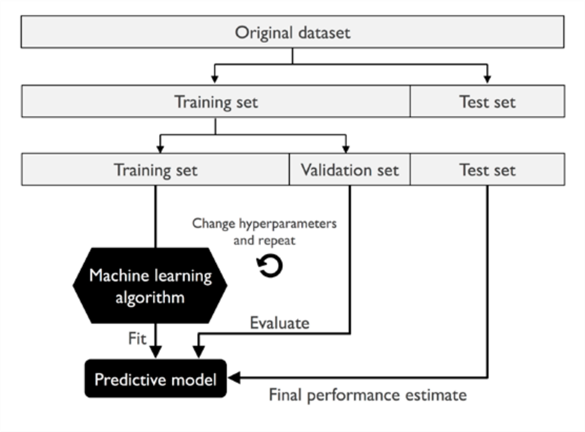
\includegraphics{./pic/chapter-4-5_pic_0.png} \emph{From S. Raschka et
al.~(see Reference)}

    \hypertarget{k-fold-cross-validation}{%
\subsubsection{k-fold Cross-Validation}\label{k-fold-cross-validation}}

    In k-fold cross-validation, we randomly split the training dataset into
k folds without replacement, where k -- 1 folds are used for the model
training, and one fold is used for performance evaluation. This
procedure is repeated k times so that we obtain k models and performance
estimates.

We then calculate the average performance of the models based on the
different, independent test folds to obtain a performance estimate that
is less sensitive to the sub-partitioning of the training data compared
to the holdout method. Typically, we use k-fold cross-validation for
model tuning, that is, finding the optimal hyperparameter values that
yield a satisfying generalization performance, which is estimated from
evaluating the model performance on the test folds. Once we have found
satisfactory hyperparameter values, we can retrain the model on the
complete training dataset and obtain a final performance estimate using
the independent test dataset. The rationale behind fitting a model to
the whole training dataset after k-fold cross-validation is that
providing more training examples to a learning algorithm usually results
in a more accurate and robust model.

    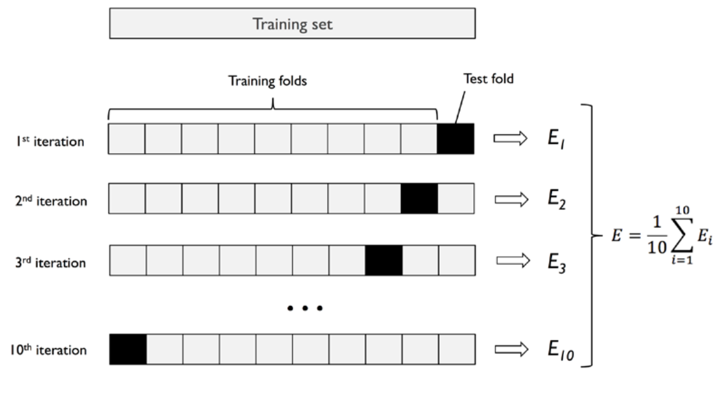
\includegraphics{./pic/chapter-4-5_pic_1.png} \emph{From S. Raschka et
al.~(see Reference)}

    \hypertarget{validation-curves}{%
\subsection{Validation Curves}\label{validation-curves}}

    

    \hypertarget{tuning-hyperparameters-via-grid-search}{%
\subsection{Tuning hyperparameters via grid
search}\label{tuning-hyperparameters-via-grid-search}}

    

    

    

    

    

    

    

    \hypertarget{references}{%
\section{References}\label{references}}

    \emph{Eryk Lewinson}, ``\textbf{Python For Finance Cookbook}'', Packt
Publishing (2020)

    \emph{Sebastian Raschka and Vahid Mirjalili} ``\textbf{Machine Learning
with Python}'', 3rd edition, Packt Publishing

    \begin{tcolorbox}[breakable, size=fbox, boxrule=1pt, pad at break*=1mm,colback=cellbackground, colframe=cellborder]
\prompt{In}{incolor}{ }{\boxspacing}
\begin{Verbatim}[commandchars=\\\{\}]

\end{Verbatim}
\end{tcolorbox}


    % Add a bibliography block to the postdoc
    
    
    
\end{document}
